\section{Phân phối Nhị thức (Binomial Distribution)}

\subsection{Định nghĩa}

Phân phối nhị thức mô tả xác suất có chính xác $k$ lần \textbf{thành công} trong $n$ phép thử độc lập, 
trong đó mỗi phép thử có xác suất thành công $p$ không đổi.  
Ta ký hiệu:
\[
X \sim \mathrm{Binomial}(n, p), \quad n \in \mathbb{N}, \; 0 \leq p \leq 1
\]


Đặt biệt, các điều kiện sau cần được thỏa:

\begin{itemize}
    \item Số lượng phép thử $n$ là cố định 
    \item Các phép thử là độc lập nhau
    \item Xác suất thành công của từng phép thử là như nhau cho mỗi lần thử
    \item Mỗi phép thử, hoặc là thành công, hoặc là không thành công.
\end{itemize}
\subsection{Probability Mass Function - PMF}

Hàm trọng lượng xác suất của phân phối nhị thức được cho bởi:
\[
P(X = k) = f(k; n, p) = \binom{n}{k} p^k (1 - p)^{n - k}, \quad k = 0, 1, 2, \dots, n
\]
với:
\[
\binom{n}{k} = \frac{n!}{k!(n - k)!}
\]
là hệ số tổ hợp, biểu thị số cách chọn $k$ thành công trong $n$ phép thử.

\subsection{Cumulative Distribution Function - CDF}

Hàm xác suất tích lũy được định nghĩa là:
\[
F(k; n, p) = P(X \leq k) = \sum_{i = 0}^{k} \binom{n}{i} p^i (1 - p)^{n - i}
\]
Không có công thức đóng cho $F(k; n, p)$, nhưng có thể tính xấp xỉ bằng hàm Beta không đều (incomplete Beta function):
\[
F(k; n, p) = I_{1-p}(n - k, k + 1)
\]
  
\begin{figure}[h!]
    \centering
    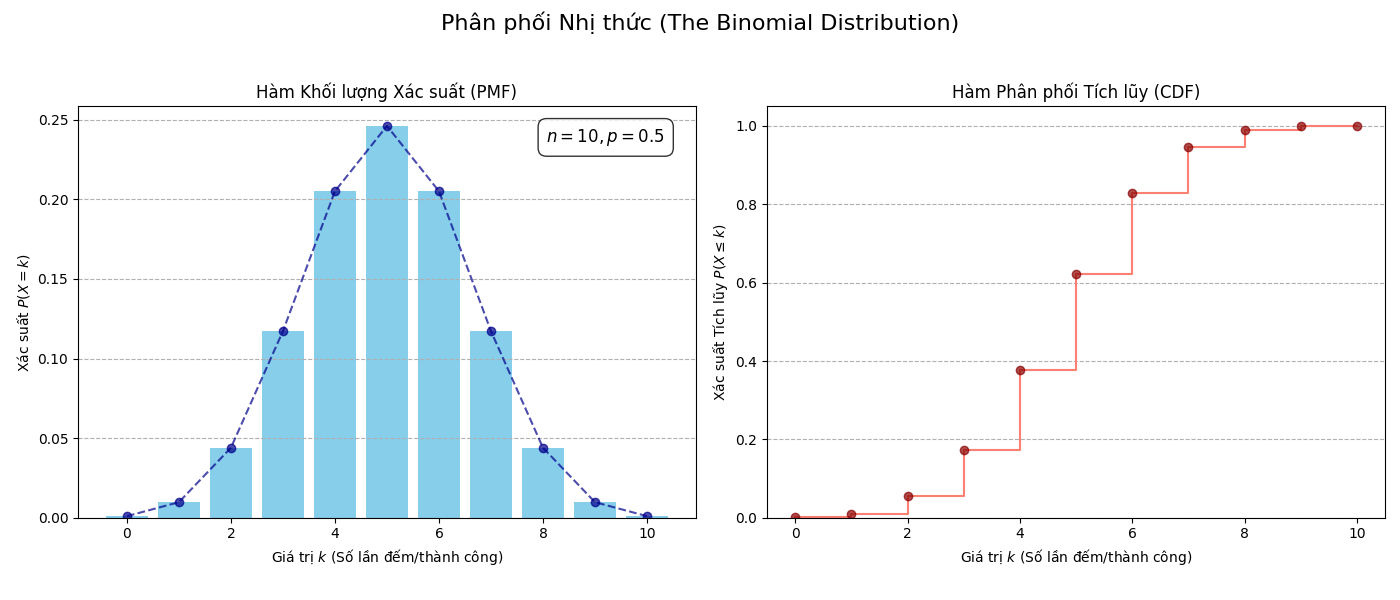
\includegraphics[width=0.8\textwidth]{images/Binomial_PMF_and_CDF.png}
    \caption{Biểu đồ Hàm Khối lượng Xác suất (PMF) và Hàm Phân phối Tích lũy (CDF) của Phân phối Nhị thức. Phân phối này mô tả số lần thành công trong $n$ phép thử độc lập.}
    \label{fig:binomial_dist}
\end{figure}
\subsection{Các đặc trưng thống kê}

\begin{itemize}
    \item \textbf{Giá trị kỳ vọng (Mean):} 
    \[
    \mathbb{E}[X] = np
    \]
    \item \textbf{Phương sai (Variance):} 
    \[
    \mathrm{Var}(X) = np(1 - p)
    \]
    \item \textbf{Mode (Giá trị có xác suất cao nhất):}
    \[
    \mathrm{mode} = \lfloor (n + 1)p \rfloor
    \]
    \item \textbf{Median (Trung vị, xấp xỉ):}
    \[
    \mathrm{median} \approx \lfloor np + \tfrac{1}{2} \rfloor
    \]
    \item \textbf{Miền xác định:}
    \[
    k \in \{0, 1, 2, \dots, n\}
    \]
\end{itemize}

\subsection{Tính chất hình dạng (Shape)}

\begin{itemize}
    \item Phân phối nhị thức là \textbf{đối xứng} nếu $p = 0.5$.  
    \item \textbf{Lệch trái (left-skewed)} nếu $p > 0.5$.  
    \item \textbf{Lệch phải (right-skewed)} nếu $p < 0.5$.  
    \item Khi $n$ lớn và $p$ không quá gần 0 hoặc 1, phân phối nhị thức có thể được \textbf{xấp xỉ bằng phân phối chuẩn (Normal Distribution)} với:
    \[
    X \approx \mathcal{N}(np, \, np(1 - p))
    \]
\end{itemize}

\subsection{Ví dụ dữ liệu và ứng dụng thực tế}

\paragraph{Ứng dụng 1: Kiểm định chất lượng sản phẩm.} 
Với số lượng các sản phẩm cho trước kết hợp với xác suất của một mặt hàng bị lỗi
Phân phối nhị thức có thể giúp xây dựng mô hình và ước lượng số lượng
mặt hàng bị lỗi, điều này giúp các nhà xây dựng sản phẩm cân nhắc về chất lượng
sản phẩm cũng như việc quản lý hệ thống, thiết bị sản xuất.

\paragraph{Ứng dụng 2: Ứng dụng trong tài chính.} 
Phân phối nhị thức đóng vai trò nền tảng trong  
\textit{Binomial Option Pricing Model} – BOPM)  
Thay vì giả định giá tài sản biến thiên liên tục (như trong mô hình Black–Scholes), 
Mô hình này giả định rằng ở mỗi bước thời gian $\Delta t$, giá tài sản cơ sở $S$ chỉ có thể:
\[
S_u = S_0 u \quad \text{hoặc} \quad S_d = S_0 d
\]
tức rằng tăng u lần hoặc là d lần
Sau $( n )$ bước (tức ta chia khoảng thời gian thành n windows và coi nó là rời rạc),
 giá cổ phiếu có thể đi qua nhiều đường khác nhau, ta có thể từ đó quan tâm đến
số lần tăng  k  trong  n  bước.
Xác suất để cổ phiếu tăng đúng  k  lần tuân theo phân phối nhị thức:

$$
P(K = k) = \binom{n}{k} p^k (1 - p)^{n-k}
$$

Từ đó, giá quyền chọn được tính bằng kỳ vọng có trọng số của các giá trị cuối cùng, với trọng số chính là xác suất nhị thức này.

$$
C_0 = e^{-rT} \sum_{k=0}^{n} \binom{n}{k} p^k (1 - p)^{n-k} , \max(u^k d^{n-k} S_0 - K, 0)
$$

Mô hình này cung cấp một cách tiếp cận rời rạc, trực quan và hiệu quả để ước lượng giá trị quyền chọn, 
đồng thời hội tụ về mô hình Black–Scholes khi $n \to \infty$.


\section{Phân phối Poisson (Poisson Distribution)}

\subsection{Định nghĩa}

Phân phối Poisson mô tả xác suất của số sự kiện xảy ra trong một khoảng cố định (thời gian, không gian, v.v.),  
nếu các sự kiện xảy ra độc lập và với tốc độ trung bình $\lambda$ không đổi.  
Ký hiệu:
\[
X \sim \mathrm{Poisson}(\lambda), \quad \lambda > 0
\]

\subsection{Probability Mass Function – PMF}

Hàm trọng lượng xác suất của phân phối Poisson là:
\[
P(X = k) = f(k; \lambda) = \frac{\lambda^k e^{-\lambda}}{k!}, \quad k = 0, 1, 2, \dots
\]

\subsection{Cumulative Distribution Function – CDF}

Hàm xác suất tích lũy được định nghĩa là:
\[
F(k; \lambda) = P(X \le k) = \sum_{i=0}^k \frac{\lambda^i e^{-\lambda}}{i!}
\]

\begin{figure}[h!]
    \centering
    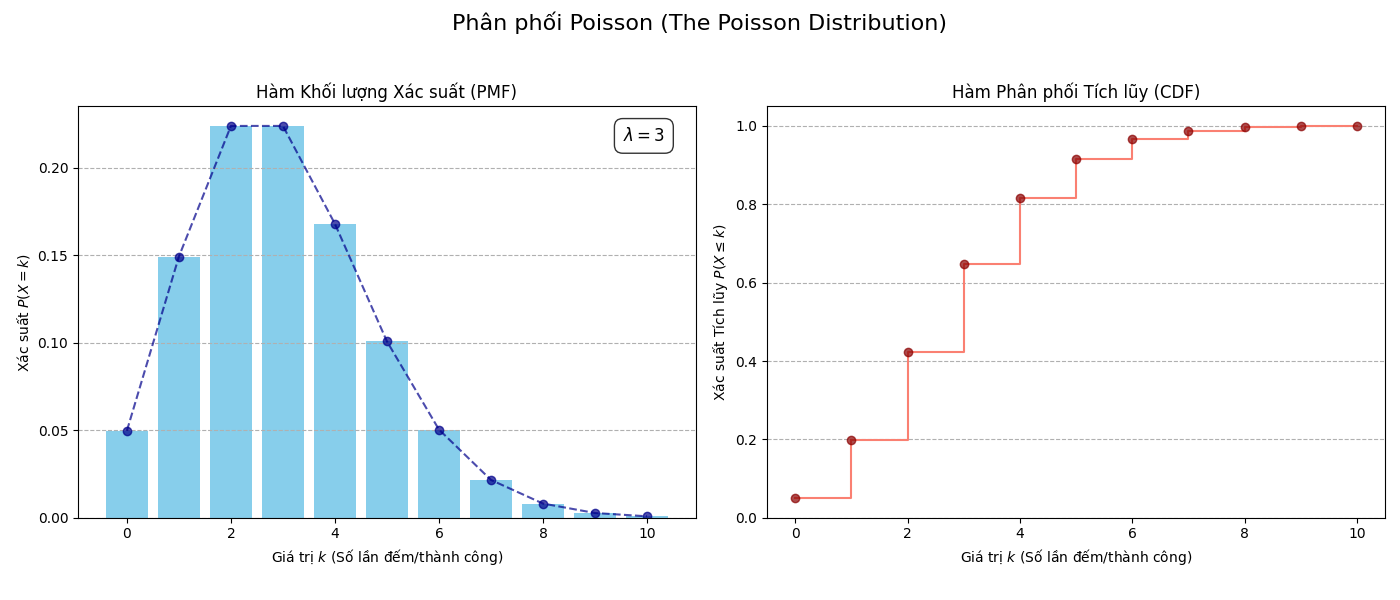
\includegraphics[width=0.8\textwidth]{images/Poisson_PMF_and_CDF.png}
    \caption{Biểu đồ PMF và CDF của Phân phối Poisson. Phân phối này mô hình hóa số sự kiện xảy ra trong một khoảng thời gian/không gian cố định, với tốc độ trung bình ($\lambda$) đã biết.}
    \label{fig:poisson_dist}
\end{figure}
\subsection{Các đặc trưng thống kê}

\begin{itemize}
  \item \textbf{Kỳ vọng (Mean):}  
  \[
    \mathbb{E}[X] = \lambda
  \]
  \item \textbf{Phương sai (Variance):}  
  \[
    \mathrm{Var}(X) = \lambda
  \]
  \item \textbf{Mode (giá trị có xác suất cao nhất):}  
  Nếu $\lambda$ không phải số nguyên, mode = $\lfloor \lambda \rfloor$.  
  Nếu $\lambda$ là số nguyên, thì có hai mode là $\lambda$ và $\lambda - 1$. 
  \item \textbf{Median (Trung vị, xấp xỉ):}  
  Không có công thức đóng chính xác; một xấp xỉ thường dùng là  
  \[
    \mathrm{median} \approx \left\lfloor \lambda + \frac{1}{3} - \frac{1}{50\lambda} \right\rfloor
  \] 
  \item \textbf{Miền xác định:}  
  \[
    k \in \{0, 1, 2, \dots\}
  \]
  \item \textbf{Hình dạng / Độ lệch:}  
  - Phân phối Poisson thường mang lệch phải (right-skewed).  
  - Khi $\lambda$ lớn, phân phối gần đối xứng và có thể xấp xỉ 
  bằng phân phối chuẩn.   
\end{itemize}
\begin{figure}[h!]
    \centering
    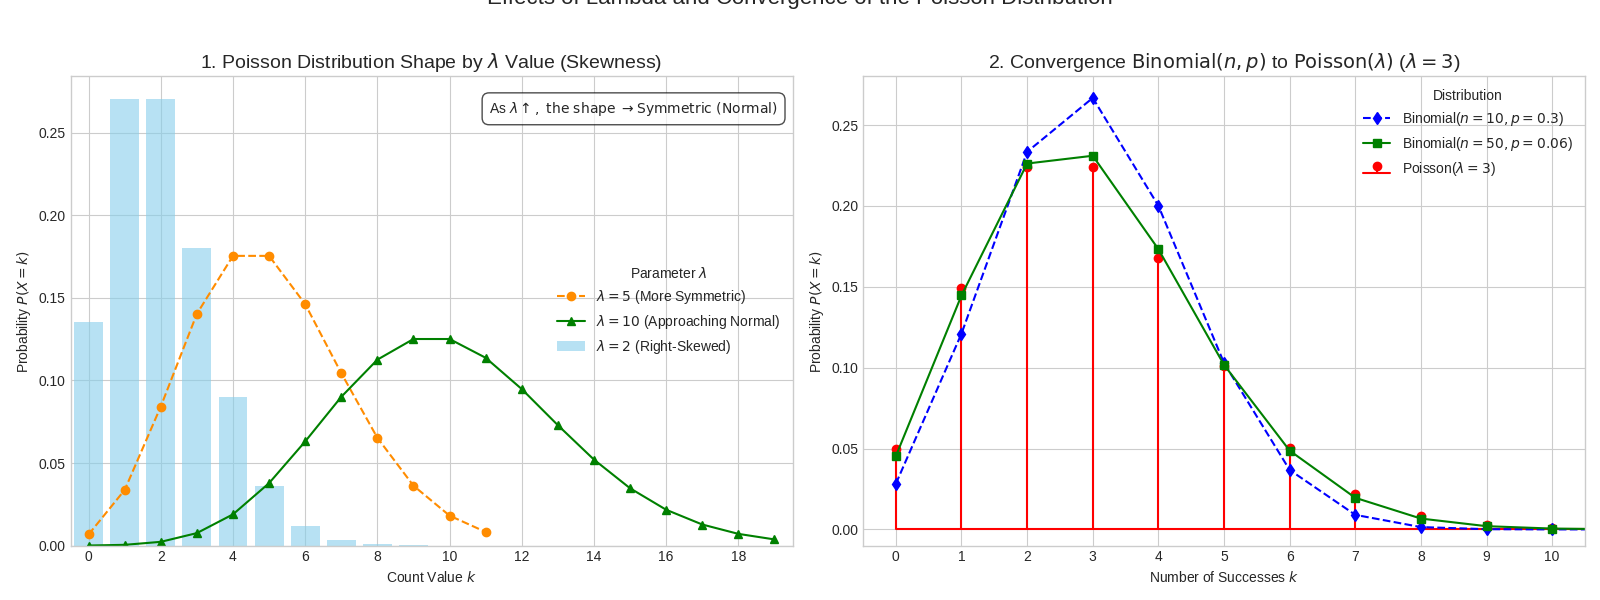
\includegraphics[width=0.8\textwidth]{images/Poisson_Shape_and_Binomial_Convergence.png}
    \caption{Hình dạng của phân phối Possion với các tham số khác nhau.}
    \label{fig:poisson_dist}
\end{figure}
\subsection{Mối liên hệ với phân phối nhị thức}


Khi $n$ rất lớn và $p$ rất nhỏ sao cho $np = \lambda$ không đổi, phân phối nhị thức $\mathrm{Binomial}(n, p)$ hội tụ về phân phối Poisson $\mathrm{Poisson}(\lambda)$:  
\[
\lim_{n \to \infty,\, p \to 0,\; np = \lambda} \binom{n}{k} p^k (1 - p)^{n-k} = \frac{\lambda^k e^{-\lambda}}{k!}
\]

\subsection*{Ví dụ dữ liệu và ứng dụng thực tế }
Phân phối \textbf{Poisson} là công cụ tiêu chuẩn để mô hình hóa 
số lần xảy ra của các sự kiện hiếm và độc lập trong một khoảng thời gian cố định.
Mà ở đây ta đề cập đến việc sử dụng để mô hình hóa Tần suất Nhấp chuột (Click Frequency)

\textbf{Mục tiêu bài toán là} dự đoán số lần ($X$) một khách hàng nhấp chuột vào quảng cáo trên trang web trong một khoảng thời gian cố định (ví dụ: 5 phút).
 Tỷ lệ nhấp chuột trung bình (mean click rate) trong khoảng thời gian đó.
 Giả định rằng các lần nhấp chuột xảy ra độc lập với một tốc độ không đổi.
Xác suất để xảy ra chính xác $k$ lần nhấp chuột được tính như sau:
    $$
        P(X=k) = (e^{-\lambda} * \lambda^k) / k!
    $$
 \textbf{Điều kiện áp dụng:} Phân phối Poisson chỉ phù hợp nếu
 \textbf{Trung bình gần bằng Phương sai} (Equidispersion). 
 Nếu \textbf{Phương sai lớn hơn cả Trung bình} (Overdispersion), thì
 \textbf{Hồi quy Nhị thức Âm} cần được sử dụng để xử lý sự khác biệt hành vi lớn giữa các khách hàng.

\section{Phân phối Nhị thức Âm}

\subsection{Định nghĩa}

Phân phối Nhị thức Âm mô tả xác suất của số lần \textbf{thất bại} ($k$) xảy ra trước khi đạt được một số lượng \textbf{thành công} cố định là $r$. Phân phối này là một giải pháp quan trọng cho \textbf{dữ liệu đếm (count data)} khi có hiện tượng \textbf{phân tán quá mức (overdispersion)} so với mô hình Poisson.

Ta ký hiệu:
\[
X \sim \mathrm{NegativeBinomial}(r, p), \quad r \in \mathbb{N}^+, \; 0 < p \leq 1
\]
Trong Data Science, nó thường được tham số hóa theo \textbf{kỳ vọng} ($\mu$) và \textbf{tham số phân tán} ($k$ hoặc $\alpha$), nơi $\mathrm{Var}(X) = \mu + \mu^2 / k$.

\subsection{Probability Mass Function - PMF}

Hàm trọng lượng xác suất của phân phối nhị thức âm (số lần thất bại $k$ trước $r$ lần thành công) được cho bởi:
\[
P(X = k) = f(k; r, p) = \binom{k + r - 1}{k} p^r (1 - p)^{k}, \quad k = 0, 1, 2, \dots
\]
với:
\[
\binom{k + r - 1}{k} = \frac{(k + r - 1)!}{k!(r - 1)!}
\]
là hệ số tổ hợp, biểu thị số cách sắp xếp $k$ thất bại và $r$ thành công trong $(k+r)$ phép thử, với phép thử cuối cùng phải là thành công thứ $r$.

\subsection{Cumulative Distribution Function - CDF}

Hàm xác suất tích lũy được định nghĩa là:
\[
F(k; r, p) = P(X \leq k) = \sum_{i = 0}^{k} \binom{i + r - 1}{i} p^r (1 - p)^{i}
\]
Giống như phân phối Nhị thức, CDF của NBD có thể liên hệ với hàm Beta không đều:
\[
F(k; r, p) = I_{p}(r, k + 1)
\]

\begin{figure}[h!]
 \centering
 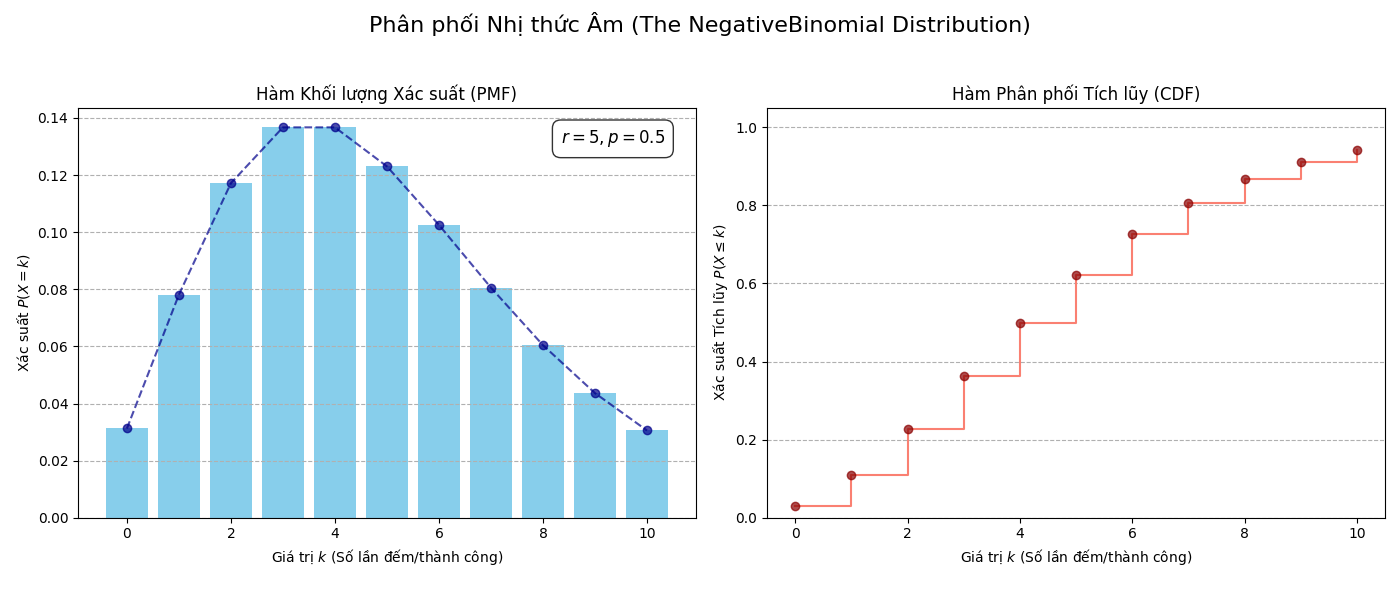
\includegraphics[width=0.8\textwidth]{images/NegativeBinomial_PMF_and_CDF.png}
\caption{Biểu đồ Hàm Khối lượng Xác suất (PMF) và Hàm Phân phối Tích lũy (CDF) của Phân phối Nhị thức Âm. Phân phối này mô tả số lần thất bại trước khi đạt $r$ thành công cố định.}
\label{fig:nbinomial_dist}
\end{figure}

\subsection{Các đặc trưng thống kê}

\begin{itemize}
\item \textbf{Giá trị kỳ vọng (Mean):} 
 $$
\mathbb{E}[X] = \frac{r(1 - p)}{p} = \mu
    $$
\item \textbf{Phương sai (Variance):} 
$$
\mathrm{Var}(X) = \frac{r(1 - p)}{p^2} = \mu + \frac{\mu^2}{r/{(1-p)}} = \mu + \frac{\mu^2}{k_{alt}}
$$
    \textbf{Lưu ý:} Phương sai luôn \textbf{lớn hơn} giá trị kỳ vọng: $\mathrm{Var}(X) > \mathbb{E}[X]$.
\item \textbf{Miền xác định:}
 $$
 k \in \{0, 1, 2, \dots\}
 $$
\end{itemize}

\subsection{Mối liên hệ với các phân phối khác}

\begin{itemize}
\item \textbf{Mở rộng của Hình học (Geometric):} Nếu $r=1$, NBD trở thành Phân phối Hình học (Geometric Distribution), mô tả số lần thất bại trước \textit{thành công đầu tiên}.
\item \textbf{Xấp xỉ Poisson:} Nếu $r \to \infty$ và $p \to 1$ sao cho $\frac{r(1-p)}{p} = \lambda$ không đổi, NBD hội tụ về $\mathrm{Poisson}(\lambda)$.
\item \textbf{Mô hình hóa Overdispersion:} Phân phối Nhị thức Âm thường được xây dựng bằng cách giả định rằng $\lambda$ (tốc độ trung bình) của phân phối Poisson không phải là hằng số mà tuân theo một \textbf{Phân phối Gamma}. Phân phối hỗn hợp (Compound Distribution) này tạo ra Phân phối Nhị thức Âm (Gamma-Poisson Mixture).
\end{itemize}

\subsection{Ví dụ dữ liệu và ứng dụng thực tế}

\subsubsection*{Bài toán Dự đoán Tần suất Mua hàng}

\textbf{Mục tiêu bài toán} là xây dựng mô hình để dự đoán \text{số lần} 
một khách hàng cá nhân sẽ thực hiện giao dịch 
(mua hàng) trong một \textbf{khoảng thời gian cố định} 
trong tương lai (ví dụ: 6 tháng, 1 năm). Dữ liệu giao dịch lịch sử của mỗi khách hàng, bao gồm:

\begin{itemize}
    \item \textbf{ID Khách hàng:} Nhận dạng duy nhất.
    \item \textbf{Số lần Mua hàng ($k$):} Tổng số giao dịch trong một khoảng thời gian quan sát.
    \item  \textbf{Các biến giải thích (Covariates):} Các đặc điểm của khách hàng ảnh hưởng đến tần suất mua (ví dụ: Giá trị đơn hàng trung bình, thời gian từ lần mua cuối cùng, nguồn gốc khách hàng).
\end{itemize}

\subsubsection*{Vấn đề của Phân phối Poisson} 
Khi cố gắng giải quyết bài toán này bằng 
\textbf{Hồi quy Poisson (Poisson Regression)}, 
họ thường gặp phải hiện tượng \textbf{Phân tán Quá mức (Overdispersion)}.
Nguyên nhân có thể do:
\begin{itemize}
    \item \text{Giả định Poisson}  Yêu cầu $\text{Mean} (\mu) = \text{Variance} (\sigma^2)$.
    \item Chênh lệch giữa người "mua sắm nhiều" và nhóm người "thi thoảng mua sắm" làm cho phương sai của dữ liệu lớn hơn rất  nhiều so với trung bình
\end{itemize}

\subsubsection*{Giải pháp: Sử dụng Phân phối Nhị thức Âm}

Phân phối Nhị thức Âm là giải pháp hoàn hảo 
vì nó có khả năng mô hình hóa sự phân tán quá mức.
Đây có thể được coi là sự kết hợp của hai phân phối:

\begin{itemize}
\item \textbf{Phân phối Poisson:} Mô tả số lần mua hàng của một cá nhân tại một tốc độ $\lambda$ nhất định.
\item \textbf{Phân phối Gamma:} Mô tả sự thay đổi của tốc độ $\lambda$ giữa các cá nhân (tức là sự không đồng nhất trong hành vi mua hàng).
\end{itemize}

Bằng cách tích hợp (compound) hai phân phối này, 
Phân phối nhị thức âm (gọi tắc là NBD) 
có thêm \textbf{Tham số Phân tán} 
(thường ký hiệu là $k$ hoặc $\alpha$) 
cho phép Phương sai lớn hơn Trung bình:

$$\mathrm{Var}(X) = \mu + \frac{\mu^2}{k}$$

(Trong đó $k$ là tham số phân tán. Khi $k \to \infty$, Phương sai $\to \mu$, và NBD hội tụ về Poisson).